%!TEX root = ../thesis.tex

\section{IMPLEMENTATION}

% ---
% Pre-processing
% ---
\subsection{Data Pre-processing}

The work was started by preparing the data, so the servers could work with it the most efficient
way. This section is devoted to the description of the initial data and how it was processed. The
section also involves comparison of deferent approaches of data structuring
and summarizing of the results.

\subsubsection{Description of the Raw Data}

The provided original data is collected using Google
Directions API~\cite{google:directions} applying following algorithm. First, on top of the city the
grid of points was constructed using WGS~84~\cite{wiki:wgs} coordinate system. Second, for every
pair of points the directions were calculated using HTTP request to the API. Returned data is
encoded in JSON format written to a text file. As result raw data is a text file where every line is
a JSON object received from Google Directions API. The process of data collection is demonstrated on
Figure~\ref{pic:collecting_data}.

\begin{figure}[ht]
  \centering
  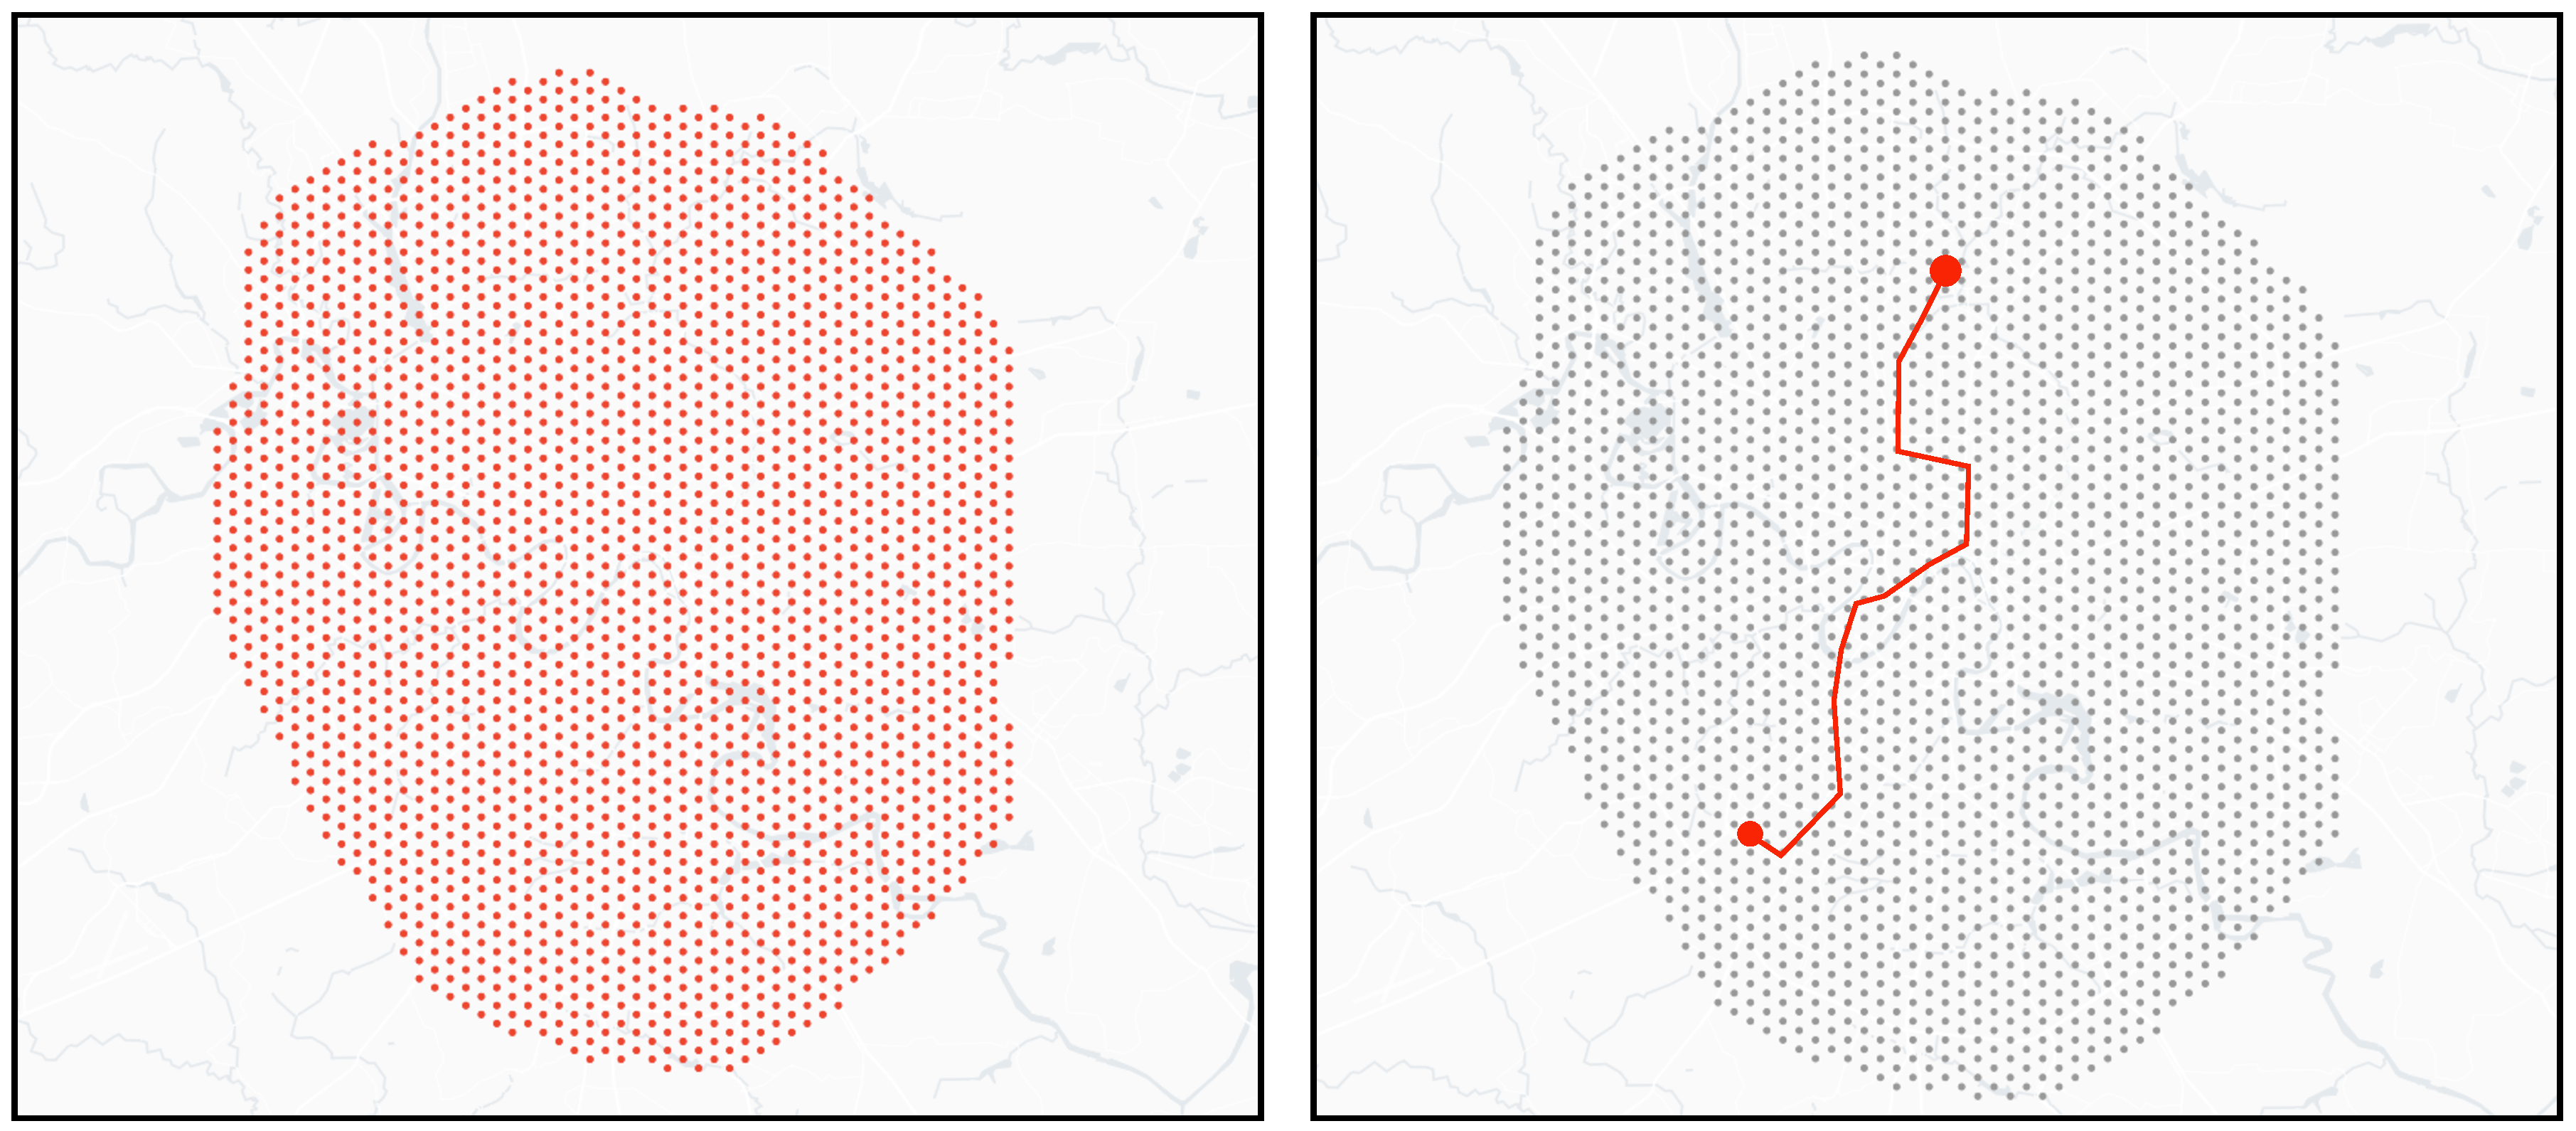
\includegraphics[width=1\textwidth]{data-collection.pdf}
  \caption{The process of the collecting data.}
  \label{pic:collecting_data}
\end{figure}

In fact there is also a meta information such as object id, job status, waypoints order,
warnings, but if we simplify and leave only important fields that we will need in pre-processing
step, then JSON object could look like this:

\begin{lstlisting}[language=json, caption=Google Directions API simplified response example,
      label={lst:google_response}]
{
  "start_lat": 55.726497,
  "start_long": 37.338183,
  "end_lat": 55.886619,
  "end_long": 37.579683,
  "data": {
    "routes": [{
      "legs": [{
        "distance": { "text": "45.1 km", "value": 45093 },
        "end_address": "Novgorodskaya ulitsa...",
        "start_address": "Razdorovskaya, Romashkovo...",
        "steps": [{
          "travel_mode": "DRIVING",
          "polyline": { "points": "wicsI{u{bFs@rDC" },
          "distance": { "text": "4.2 km", "value": 4166 },
          "duration": { "text": "7 mins", "value": 438 }
        }, ... ]
      }, ... ]
    }, ... ]
  }
}
\end{lstlisting}

As it can be seen from simplified response example, the object contains coordinates of the start and
end point, array routes which consists of \texttt{legs}. \texttt{Legs} are parts of the route
between waypoints. Since in our queries we do not have middle waypoints, the routes array will have
only one element in all cases. Each leg contains total distance information about start and end
location. Also, inside \texttt{legs} there are \texttt{steps}, each step is a part of route which can
be described by single command and type of transport, for example ``move forward by bus'' is clearly
a step. Step keeps information about its distance and duration which will be needed to complete this
step. Other important things are \texttt{travel\_mode}, which indicates what type of transport is
used in this step, and \texttt{polyline}, which is essentially a set of points of points encoded using
lossy Google's algorithm that converts array of float numbers, first, to binary representation, then
to decimal integers and, finally, to string using ASCII codes~\cite{google:polyline}.

\subsubsection{Extracting Points}

The data collection was initiated before by Mathrioshka LLC thus the first task was extracting
grid points from the raw data. This step was performed utilizing set script written in Python, which
is reading file line by line and extracting starting location point from the data. The
idea of the algorithm is presented in Listing~\ref{lst:points_extraction}. As can be seen from
the listing, Geohash~\cite{wiki:geohash} standard was used to prevent repetitions of the points.
Thus, coordinates could be mapped to strings which can be utilized as ids in points dictionary.
In our implementation for encoding \lstinline{python-geohash} library was used~\cite{pip:geohash}.
For storing, the result of the algorithm the pickle~\cite{pickle} format was selected, since it has
quite simple interface and built into Python standard library.

\begin{lstlisting}[language=python, caption=Points extraction, label={lst:points_extraction}]
points = []

for line in jsonfile:
    json_obj = json.loads(line)
    slat = json_obj['start_lat']
    slng = json_obj['start_long']
    point = {
        'point_id': geohash.encode(slat, slng),
        'lat': slat,
        'lng': slng
    }
    points[point['point_id']] = point
\end{lstlisting}

\subsubsection{Extracting Lines}

Another important task was to extract lines from the file, but first to make experiments faster
it was decided to convert data to more convenient format hence it would be easier to
experiment and process data more effectively. Once we have data extracted, we will convert it
to the set of GeoJSON files and after that generate vector tiles which will be served by our
tile server.

For intermediate lines representation the CSV file format was selected due to its simplicity
and availability of the encoders and decoders inside standard Python library. The algorithm is
presented in Listing~\ref{lst:lines_conversion}. First, we initialize table of lines which will
contain all unique lines encoded in raw data. Second, we read file object by object. Each object
is then decomposed into set of lines using \lstinline|lines_from_json()| function. Once lines are
extracted the assertion is performed to check whether the line was already met before. If the
answer is no, then we initialize line, otherwise we just sum distance and duration
and increase the weight by one. The distance, duration and weight are necessary to compute
line width, speed, prevailing transport and accessibility of the point.

%%%
% TODO:
% Add description of lines_from_json()
%%%

\begin{lstlisting}[language=python, caption=Lines conversion., label={lst:lines_conversion}]
# Table of lines
T = {}

with open(DATA_PATH) as jsonfile:

    for json_str in jsonfile:
        json_obj = json.loads(json_str)

        for line in lines_from_json(json_obj):
            line_hash = line['line_hash']

            if line_hash not in T:
                del line['line_hash']
                T[line_hash] = line
                T[line_hash]['line_id'] = len(T)
            else:
                T[line_hash]['weight'] += 1
                T[line_hash]['distance'] += line['distance']
                T[line_hash]['duration'] += line['duration']
\end{lstlisting}

\subsubsection{Link Lines to Points}

Since we have our data extracted, now it is important to have references from lines to points. The
first approach was to store in the CSV file containing lines also point identifiers thus in case we
would need to get all lines for given points we would just go through the lines table an select only
those lines which have ID of the point. It was revealed that this approach is quite slow since each
line can be associated with up to 2000 points and it would take $O(N \times M)$ time complexity to
get all lines where $N$ is the size of the lines table and $M$ the length of the array points. The
second approach was to store lines identifiers inside points table what resulted in significant
improvement and we could access all lines for $O(N)$. In combination with Pandas
library~\cite{pandas}, which is used for storing lines table in memory, method with storing lines in
points table results in even more considerable speed improvement. On the other hand, the points
dictionary grew in size and started to occupy more than 8 GB of the disc space. To overcome this
issue the shelve~\cite{shelve} data type was chosen. Shelve is a simple file-based database with
object-like interface, which is fully compatible with pickle. Thus without serious code
modifications the memory usage was dropped from 8 GB to 200 MB.

\subsubsection{Transformation to Vector Tiles}

Once the data is transformed to convenient form, the next step is convert it to vector tiles.
For this purpose the tippecanoe~\cite{tippecanoe} tool was selected which is developed by Mapbox team
as open source project. The drawback of this instrument is that to generate tiles with several
layers one would need to have separate GeoJSON file for each tile layer. In our application we will
need 128 tile layers to render all weights, colors and also apply filtering. Thus, we first need to
generate 128 GeoJSON files for each point and then we could easily convert set of GeoJSON files to
tiles.

\subsubsection{Results}

The resulting preprocessing scheme is demonstrated on Figure~\ref{pic:transforming_data}.
First, we transform raw data to intermediate state which is shelve of points with links to lines
and table of lines with properties. Next, for each point we generate a folder which contains
GoeJSON file describing set of lines associated with given point (all directions from one point on the grid
to others), then GeoJSON files are transformed to vector tiles. In course of the preprocessing
there were other approaches, for instance when rendering was not utilizing vector tiles, but
just GeoJSON files there were an improvement which allowed merging adjacent lines together to reduce
the size of the occupied space, but once the the implementation started to be based in MBTiles lines
merging was rejected. It is important to note that initially the tiles generation was
planned to implement in real time, but it was discovered that real-time processing takes significant
amount of time which results in delays in server responses.

\begin{figure}[h]
  \centering
  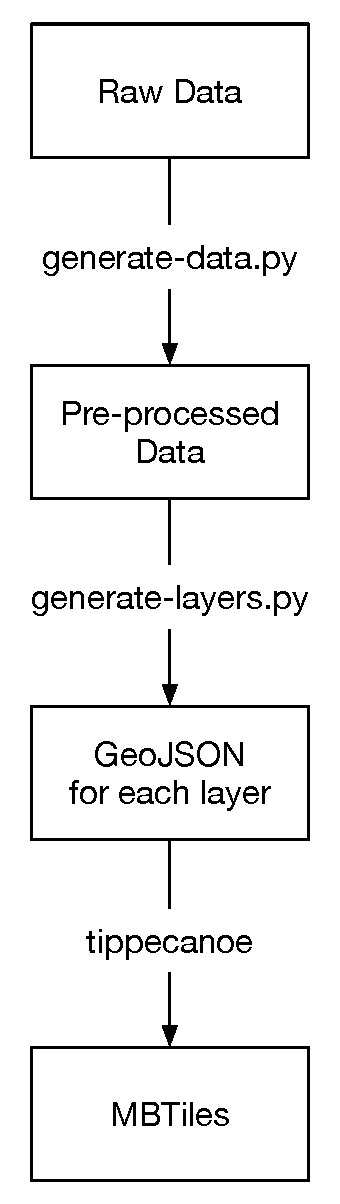
\includegraphics[width=.25\textwidth]{data-transformation.pdf}
  \caption{The process of the data transformation.}
  \label{pic:transforming_data}
\end{figure}

% ---
% Client
% ---
\subsection{Web Interface}

In this section the main architectural pattern used for building the interface is described
including diagrams showing hierarchy of components, the selection of map drawing library is made.

\subsubsection{FLUX Architecture}

In the process of the development of the web interface the crucial thing is the state management. In
2010 the Backbone.js~\cite{backbone} library was introduced which was supposed to solve the problem
of the state management often applying MVC~\cite{backbone:mvc} pattern. Although, on large projects
there where a lot of cross-dependencies and this paradigm resulted to be hard to maintain. Later in
2013 Facebook~Inc. introduced component based React~\cite{react} library which allowed to think of
the interface as function which maps state to representation. Although, React was implemented only
as library for creating views and was not meant to solve problem of data state management in the
application it still had significant success. In 2014 Facebook~Inc. suggested FLUX~\cite{flux}
pattern which gained significant popularity. The idea behind FLUX can be described as follows: data
comes from the store to the view which renders it, the user can fire an action, for example by
pressing a button, the action is goes to the dispatcher which tells to all of the stores that
certain action was fired. The stores modify the data and broadcast it to all of the views which are
subscribed to this store. All of the views that received new data gets re-rendered. The illustration
of this process can be seen on Figure~\ref{pic:flux}.

\begin{figure}[h]
  \centering
  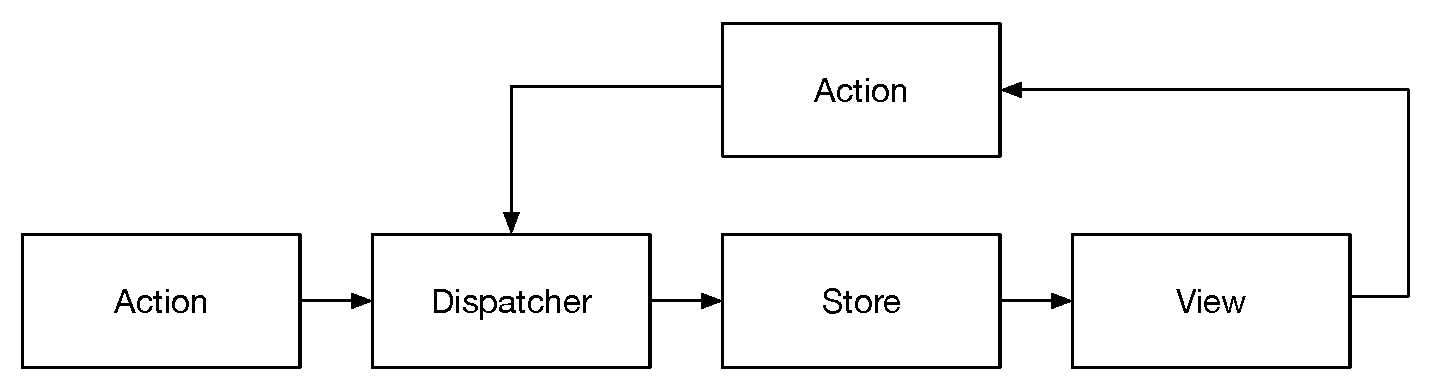
\includegraphics[width=.8\textwidth]{flux.pdf}
  \caption{FLUX architecture.}
  \label{pic:flux}
\end{figure}

Eventually FLUX evolved in library called Redux~\cite{redux}, which introduced few important
modifications such as suppressing dispatcher, using pure functions for data modifications, using
only single store where all of the data is accumulated, introducing middlewares for managing
side effects. All this features create easier debugging experience and clear separation
of concerns. Thus, for the development Redux and React libraries were chosen.

React components were organized as it is illustrated on Figure~\ref{pic:comp-diag} accordingly to
the approach of presentational and container components~\cite{redux:ppc}. The main presentational
component is \texttt{App} which is the only one connected to the store directly. All other
components are ``dumb'' and receive data as well as actions which are needed to be fired from
\texttt{App}. The \texttt{SpeedMapButton} represents a switch for choosing between coloring lines by
speed and by the type of transport. The \texttt{Map} components accumulates all of the logic related
to drawing maps. The \texttt{TransportFilter} shows what kind of transport should be displayed on
the map using set of \texttt{TransportCheckbox}. The \texttt{LocationSelector} shows
information about selected location. The \texttt{ModeSelector} switches between global overview and
location information. The \texttt{OverviewModeSelector} is needed to switch states
while being in overview mode. The \texttt{ReactSlider} is a third-party component utilized
for filtering by transport speed and accessibility coefficient. The positioning of all of
the components is illustrated on Figure~\ref{pic:comp-screen}.


\begin{figure}[ht]
  \centering
  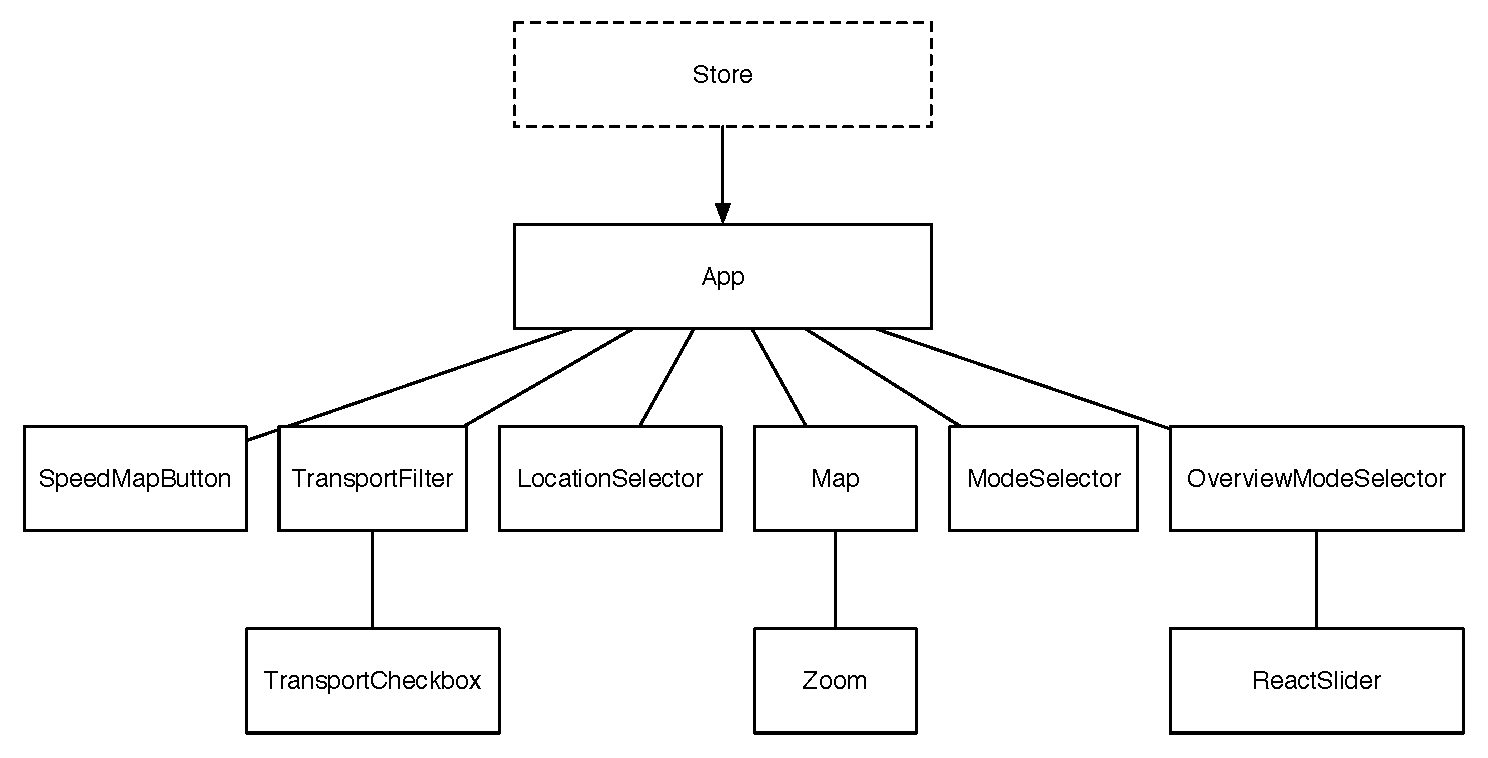
\includegraphics[width=1\textwidth]{components.pdf}
  \caption{Structure of the components}
  \label{pic:comp-diag}
\end{figure}

\begin{figure}[ht]
  \captionsetup{justification=centering,margin=1cm}
  \centering
  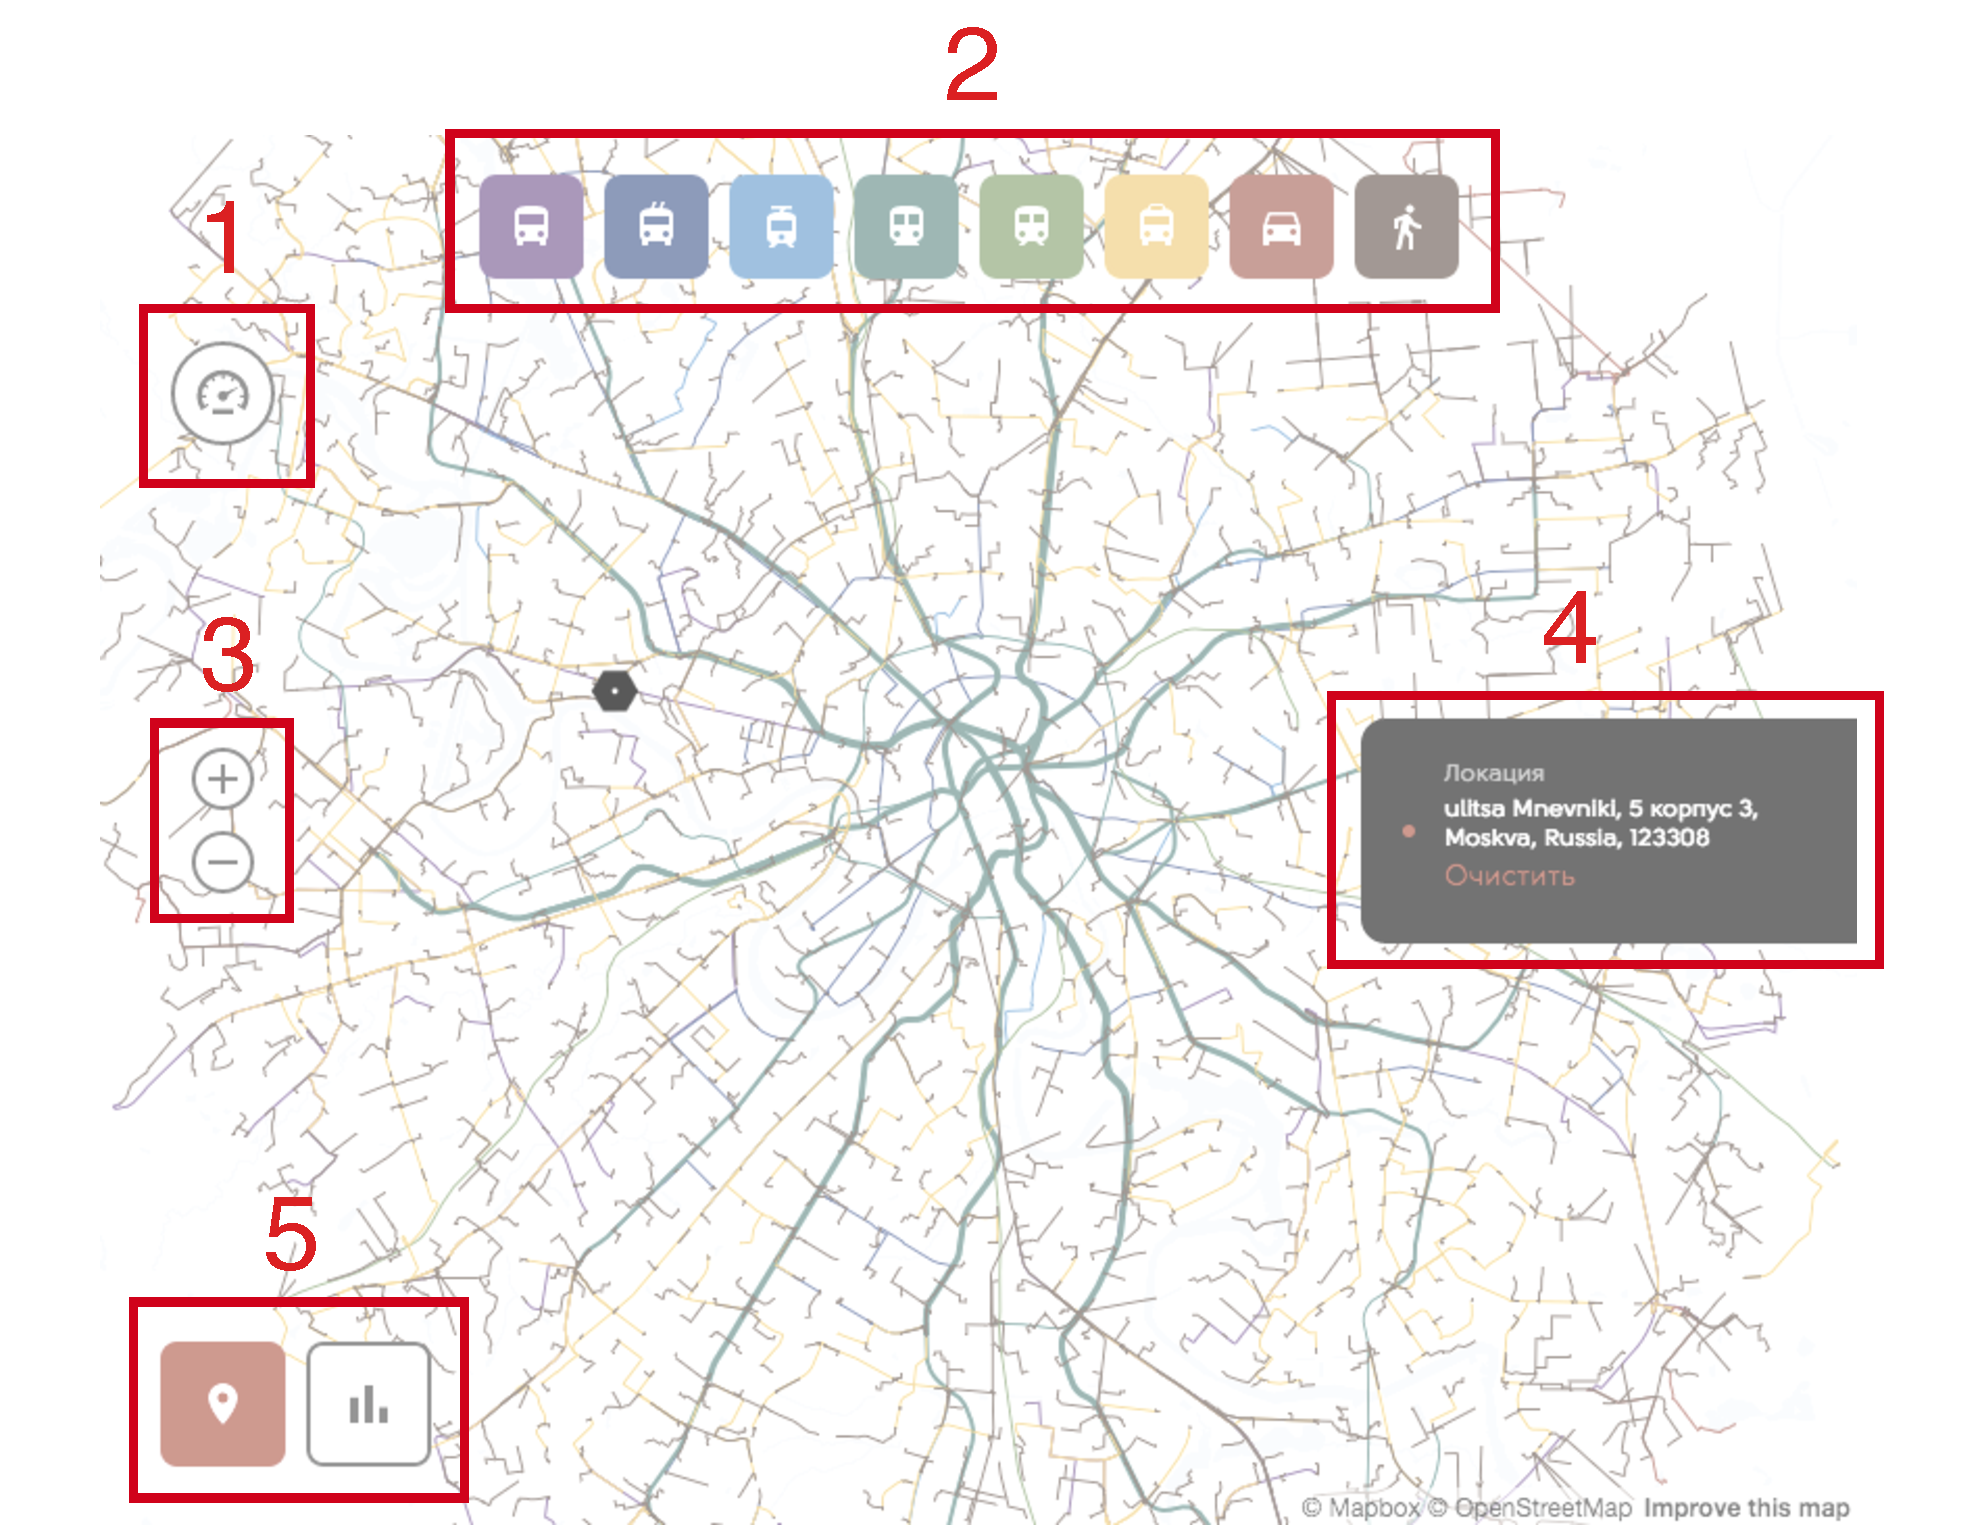
\includegraphics[width=.6\textwidth]{components-1.pdf}

  \par \vspace{0.5cm}

  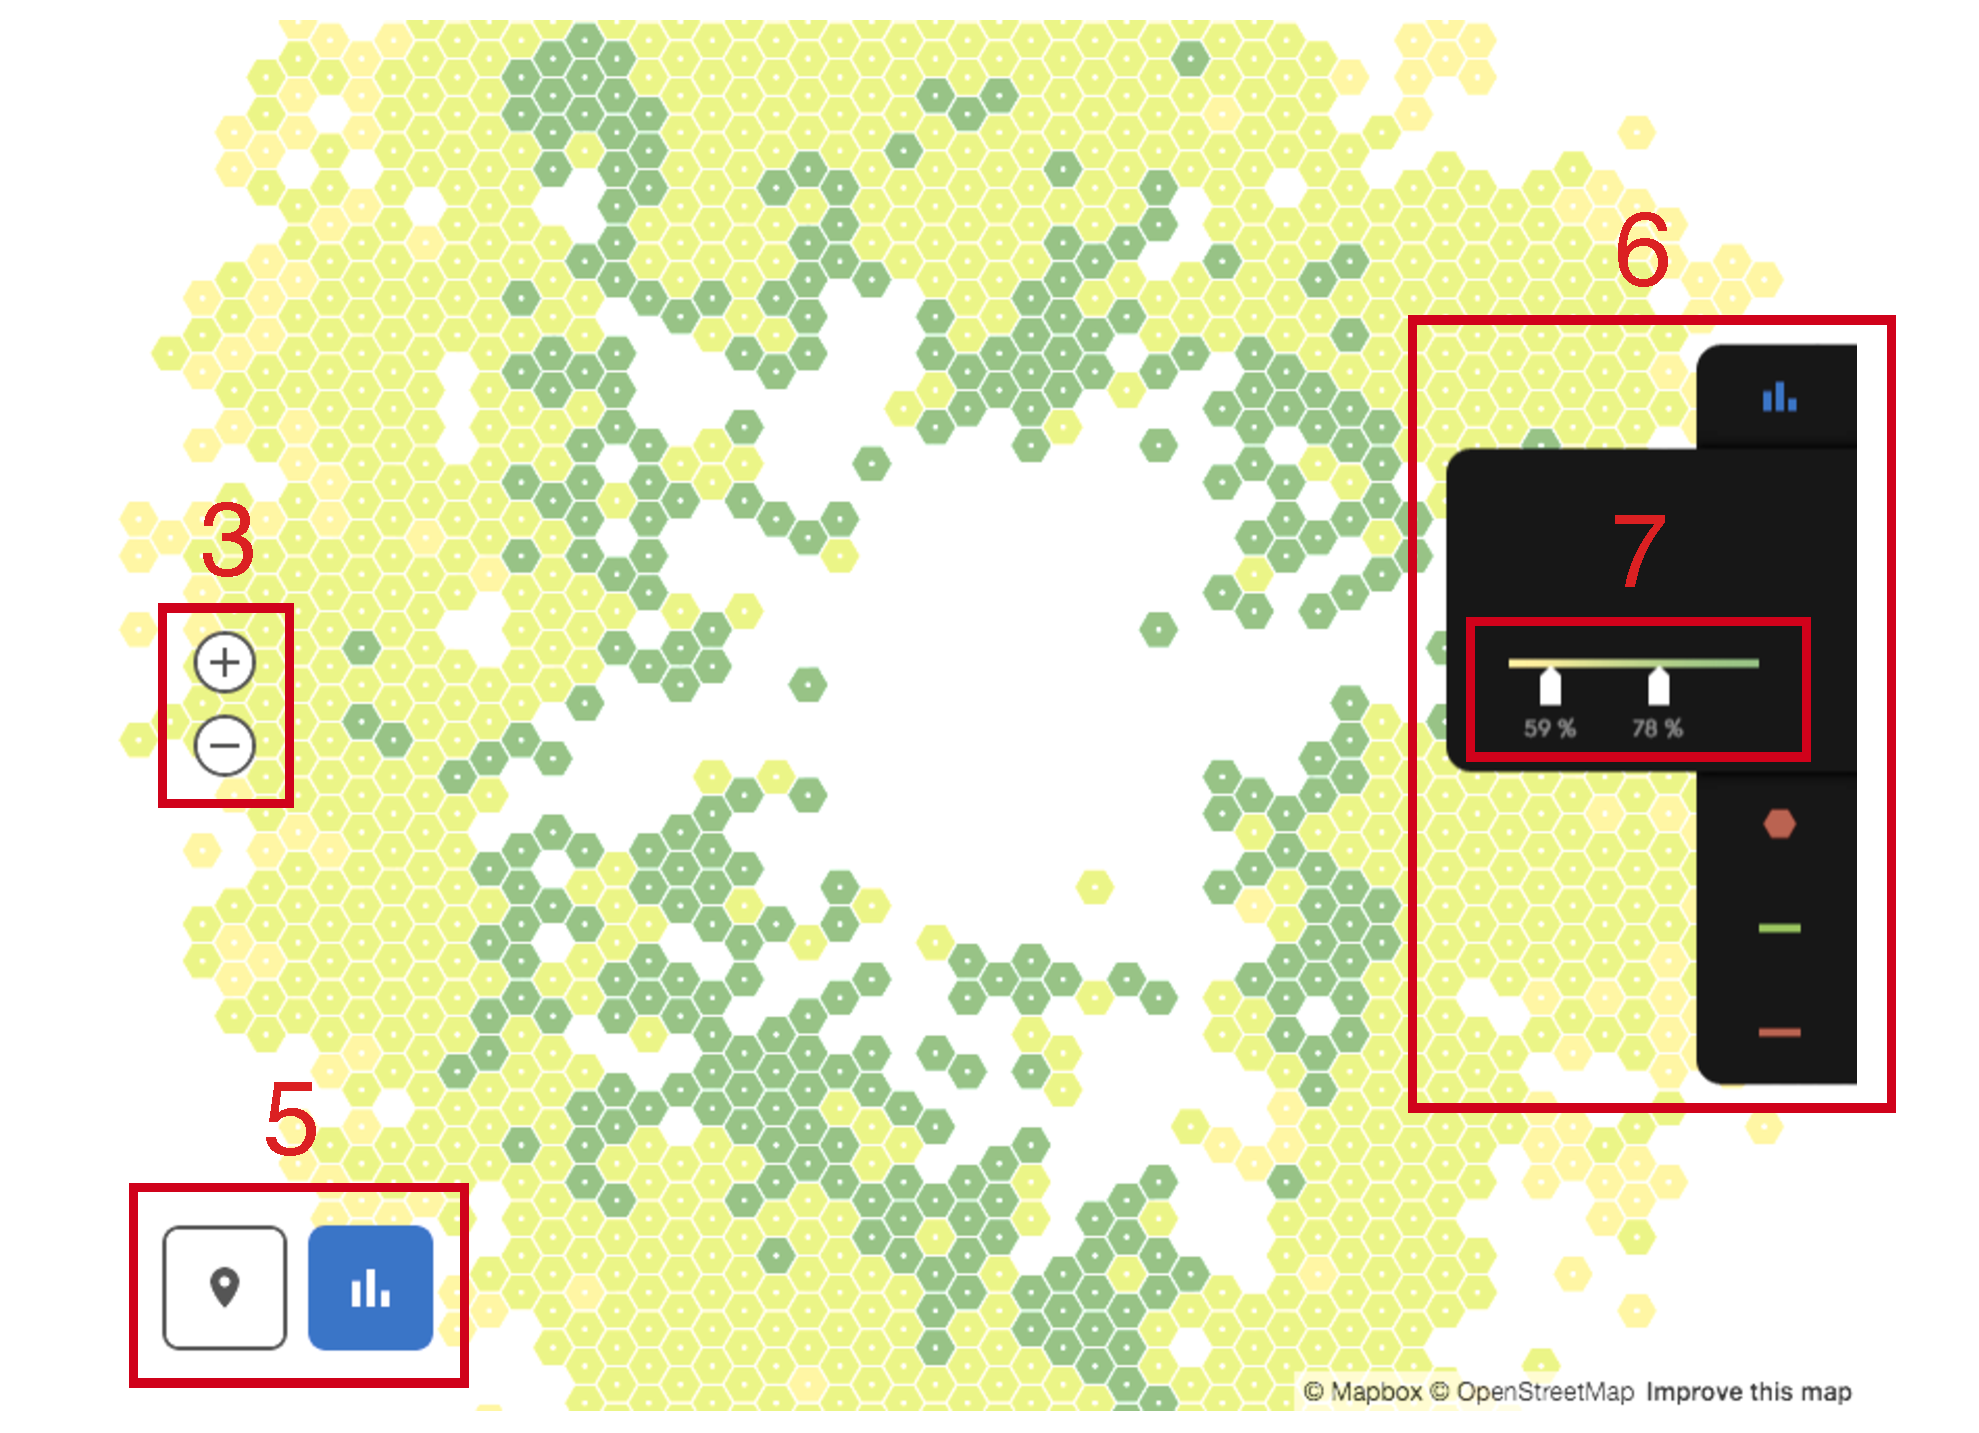
\includegraphics[width=.6\textwidth]{components-2.pdf}
  \caption{Components positioning. 1 -- SpeedMapButton; 2 -- TransportFilter; 3 -- Zoom;
  4 -- LocationSelector; 5 -- ModeSelector; 6 -- OverviewModeSelector; 7 -- ReactSlider.
  }
  \label{pic:comp-screen}
\end{figure}


\subsubsection{Drawing Maps}

As it was described before, there are several the most famous libraries for drawing maps
such as Yandex Mapx, Google Maps, Leaflet.js and Mapbox GL JS. To determine which library will
suite better for our program, the needed functionality should be defined. The most important
features are:

\begin{enumerate}
  \item Panning and zooming.
  \item Support vector tiles.
  \item Rendering map from external data source.
  \item Support of the vector tiles styling of such properties as line widths, line colors.
  \item Ability to render icons at certain location.
  \item Support for map styling.
  \item Uses open standards.
\end{enumerate}

Among all of the libraries the most suitable is Mapbox GL JS which supports all of the listed
features. Although some part of the free Mapbox toolkit has limitations, for example free
subscription plan allows not more than 50000 map views per month, but for our project that was
enough. Moreover, later the tile source can be replaced with completely free solution and hosted
locally. Important to note that Mapbox uses OpenStreeMap for geographical data provider which is
free to use. As for Google Maps and Yandex Maps, they were not supporting maps from external data
sources which is needed for rendering custom vector tiles. Although Leaflet is a very popular choice
for map drawing, it is not suitable for our particular application since it does not support vector
tiles rendering.

\subsection{Tile Server}

For rendering all of the directions the tile server would need to be chosen. The tasks
in our application for this component are quite trivial:

\begin{enumerate}
  \item Fast.
  \item Support of the MBTiles format.
  \item Easy to setup and configure.
  \item Free and open-source.
\end{enumerate}

The great candidate for this role was Tessera tile server~\cite{gh:tessera} which is written in
Node.js and based on Tilelive interface (developed by Mapbox). Moreover, Tessera
is really easy to install using npm package manager. The configuration file should be
written in JSON format and can be easily generated from our data. The only needed parameters
are source path to the data and the URL on which particular vector tiles will be available.

\subsection{RESTful Server}

For the server implementation Python language and its ecosystem were utilized. Since Python was
already used for pre-processing to reduce the amount of different languages it was decided to
continue to work with Python for server implementation as well, however the web framework for
serving data should be chosen. Two main options were considered such as Flask~\cite{flask} and
Bottle~\cite{bottle}. The API has only one resource for serving points which makes server very
simple. However, both Flask and Bottle are suitable for this task, the Bottle was chosen since it is
simpler and does not have any other dependencies. On the other hand, Flask is more powerful and
provides wider set of tools but for this particular task it is redundant.
